\documentclass[10pt]{IEEEtran}

\usepackage[utf8x]{inputenc}
\usepackage[L7x]{fontenc}
\usepackage[lithuanian]{babel}
\usepackage{listings}
\usepackage{graphicx}
\usepackage{epstopdf}


\lstset{
    basicstyle=\footnotesize,
    language=Java,
    morekeywords={String,each,in,Iterator}
}

\author{Maksim Norkin\\ \texttt{maksim.norkin@ieee.org}}
\title{Modernios informacinės sistemos\\Dalis 1}

\begin{document}

    \maketitle

    \section{Laboratorinis darbas nr 1.\\Dalykinės srities pasirinkimas}

        \subsection{Užduotis}

            Dalykinę sritį aprašyti žodžiais ir pavaizduoti paveikslėlyje. Būtina bendrai aprašyti vykstančius verslo procesus. Ta pati pasirinktoji dalykinė sritis turi būti nagrinėjama visuose  tolimesniuose darbuose. 

            Reikia pateikti pasirinktos dalykinės srities aprašymą. Aprašymas turi būti tekstinis ir iliustruotas vaizdžiuoju paveikslėliu. Aprašymui sudaryti turi būti naudojami dalykinės srities  terminai. Aprašymas turi atspindėti pagrindinius dalykinės srities aktorius, procesus bei įmonės veiklą įtakojančius išorinius agentus. Aiškiai turi būti išryškinta probleminė sritis, kuri parodo, kodėl yra svarbu nagrinėti pasirinktą dalykinę sritį. 

            Taip pat gali būti vaizduojami informaciniai srautai, materialiniai srautai, sistemos veiklą  kontroliuojantys elementai, dalyvių požiūriai ir emocijos, konfliktinės situacijos. Turi būti pateikta vaizdžiojo paveikslėlio specifikacija.

        \subsection{Įvadas}

            Dalykinė sritis pasirinkimas padaromas automobilių stovėjimą teikiančios įmonės naudai. Padarius šios srities analizę, nuspręsta, kad šioje srityje galima darbą optimizuoti galinio kliento naudai.

        \subsection{Analizė}

            Iškeliama problema yra randama kiekvienos dienos situacijoje, kuomet tik važiuojame į bet kokio pobūdžio susitikimą ir reikia automobilį palikti stovėjimo aikštelėje.

            Struktūrinė automobilių stovėjimo paslaugų teikimo įmonė schema pavaizduota \ref{fig:struktura} pav. Jos sudarančių struktūrinių vienetų funkcijos ir ryšiai yra pateikti \ref{table:struktura} lentelėje. 

            Vienas iš problematiškiausių mazgų, yra ryšys tarp kliento ir terminalo. Jam užtikrinti reikalingas patikimas ryšys tarp banko, telekomunikacijų bendrovės, techninės priežiūros specialisto ir pavedimų posistemės vientiso veikimo. Esamą posistemę būtina suprastinti, kadangi neveikiant vienam iš posistemės mazgų -- griūna visos posistemės darbas.

            \begin{figure*}[t]
                \centering
                \includegraphics[width=500px]{figures/struktura.eps}
                \caption{Dalykinės srities struktūra.}
                \label{fig:struktura}
            \end{figure*}

            \begin{table*}[t]
                \centering
                \renewcommand{\arraystretch}{1.3}
                \caption{Dalykinės stuktūros paaiškinimas}
                \label{table:struktura}
                \begin{tabular}{|c|p{5cm}|p{5cm}|} \hline 
                    \textbf{Schemos objektas} & \textbf{Objekto aprašymas, funkcijos} & \textbf{Ryšiai su kitais objektais} \\ \hline

                    Direktorius & 
                    \begin{itemize} 
                        \item Darbo našumo gerinimas 
                        \item Darbo metodikos prižiūrėtojas 
                        \item Terminalų plėtra
                    \end{itemize} & 
                    \begin{itemize}
                        \item Leidimų išdavimo derinimas su savivaldybe 
                        \item Projektų derinimas su architektu 
                    \end{itemize}\\ \hline

                    Architektas & 
                    \begin{itemize}
                        \item Projektų terminų derinimas
                        \item Darbų paskirstymas
                        \item Darbo metodikos tiesioginė priežiūra 
                    \end{itemize} & 
                    \begin{itemize}
                        \item Darbo paskirstymas sistemų inžinieriui
                        \item Sistemos priežiūros darbai su administratoriumi
                    \end{itemize} \\ \hline

                    Administratorius &
                    \begin{itemize} 
                        \item Serverių priežiūra
                        \item Pavedimų saugumo užtikrinimas
                        \item Bankinės sistemos diegimas
                    \end{itemize} &
                    \begin{itemize}
                        \item Atnaujinimų priėmimas iš sistemų inžinieriaus
                        \item Atnaujinimų įgyvendinimas serveryje
                    \end{itemize} \\ \hline

                    Sistemų inžinierius &
                    \begin{itemize} 
                    \item Sprendimų įgyvendinimas
                    \item Optimaliausių sprendimų taikymas
                    \end{itemize}& 
                    \begin{itemize}
                    \item Darbų derinimas su architektu
                    \item Darbų koordinavimas su administratoriumi
                    \item Atnaujinimo parengimas administratoriui
                    \item Bankinių protokolų įgyvendinimas
                    \end{itemize}\\ \hline

                    Techninės priežiūros inžinierius &
                    \begin{itemize}
                    \item Terminalų priežiūra
                    \end{itemize} & 
                    \begin{itemize}
                    \item Darbų derinimas su telekomunikacijų bendrovėmis
                    \item Ryšio užtikrinimas su terminalu
                    \item Administratoriaus pagalba
                    \end{itemize}\\ \hline

                    Klientas &
                    \begin{itemize} 
                    \item Paslaugų naudojimas
                    \item Laiko ribų įsipareigojimas
                    \end{itemize}& 
                    \begin{itemize}
                    \item Kreipimas į terminalą
                    \item Apmokėjimo patvirtinimo gavimas
                    \end{itemize}\\ \hline
                \end{tabular}
            \end{table*}

        \subsection{Išvados}

            Laboratorinio darbo metu buvo išnagrinėta dalykinė sritis ir pažymėta jos pagrindinė probleminė sritis. Pateikta dalykinės srities struktūros schema, bei jos funkcinis ir ryšių aprašymas. Būtina optimizuoti ir suprastinti kliento naudojimosi terminalu sistema ir ją suprastinti, kadangi keturių mazgų sistema gali būti labai nepatikima.

    \section{Laboratorinis darbas nr. 2}

        \subsection{Užduotis}

            Verslo sistemos tikslų modeliavimas. Apibrėžti strateginį tikslą ir operacinius tikslus, nurodyti jų hierarchinius ryšius. Tikslas nurodo siekiamą būseną. Tikslai gali būti kiekybiniai (pamatuojami) ar kokybiniai.

            Kiekvienam kiekybiniam tikslui nurodyti:

            \begin{itemize}
                \item Koks jo matavimo vienetas
                \item Kokia esama vertė
                \item Per kokį laikotarpį reikia nurodytą vertę pasiekti
            \end{itemize}    

            Žemiausio lygmens operacinio lygmens tikslams nurodyti:

            \begin{itemize}
                \item Problemą(-as), kurios trukdo tą tikslą įgyvendinti
                \item Problemos priežastį
                \item Veiksmą, kuris nurodo problemos sprendimo strategiją
                \item Uždavinius, kurių įgyvendinimas padeda išspręsti problemą
            \end{itemize}

            Tikslų ir/ar problemų, priežasčių, veiksmų ir uždavinių hierarchinę struktūrą galima atvaizduoti, naudojant UML klasių diagramą.

        \subsection{Įvadas}

            Verslo sistemos strateginis tikslas yra kuo žemesnės laikinės sąnaudos, užtikrinant tokį patį ir didesnį kokybės lygį. Vienas iš strateginių tikslų yra ir inovacijų diegimas. Versle naujovės ir inovacijos yra didžiausias plėtros ir pajamų šaltinis.

        \subsection{Analizė}

            Kliento pusė automobilio stovėjimo paslaugomis nori naudotis greitai, patogiai ir efektyviai. Klientas turi jausti ne grėsmę, kad jo automobilis buvo paliktas gatvėje neprižiūrėtas, tačiau saugumo jausmą ir užtikrintumą, kad jo atlikta operacija ne tik leidžia jam statyti automobilį tam skirtoje vietoje, tačiau ir užtrina tolimesnį paslaugų gerinimą.

            Viena iš inovacijų gali būti pilnai automatizuota automobilių stovėjimo apmokėjimo sistema, kuriai visiškai nereikia terminalų. Jis, kaip toks fizinis objektas, yra perkeliamas į telekomunikacijų bendrovę fundamentaliai. Klientas, turintis glaustus santykius su savo ryšio operatoriumi, telefono pagalba užregistruoja savo automobilio numerį kaip stovėjimo aikštelės naudotoją ir mobilios programos pagalba užfiksuoja nuo kada prasidėjo automobilio stovėjimas. Jokio laiko limito nėra taikoma -- klientas stovi tiek, kiek reikia, apvalinant stovėjimą iki minučių tikslumo. Klientui užfiksavus, kad jos naudojamas automobilis paliko stovėjimo vietą, jis informuoja operatorių. Operatorius pilnai žino kurioje vietoje ir kuriam laiko tarpui klientas buvo palikęs savo naudojamą automobilį.

            Remiantis tokia galinio kliento schema, automobilių stovėjimo įmonė turi tik pateikti telekomunikacijų bendrovei stovėjimo įkainius, priklausomai nuo stovėjimo zonų, kurios yra suderinamos su savivaldybe. Terminalų nebūvimas priveda prie to, kad galima ne tik sumažinti techninės priežiūros inžinieriaus pareigų aibę, tačiau ir visiškai jį pašalinti iš nagrinėjamos įmonės schemos. Iš darbo perskirstymo, techninės priežiūros inžinierių galima kvalifikuoti į testuotoją, kuris užtikrintų sistemų inžinieriaus pateikiamų sprendimų kokybės lygį. 

            Kita inovacija, tai šiuolaikinės automatizuotos atnaujinimo sistemos, kurios nebereikalauja atskiro žmogaus, kuris užsiima būtent šituo darbu. Tas pas liečia ir serverio priežiūros darbus. Taip iš įmonės sistemos iškrenta kaip toks administratorius. Tai padidina sistemų inžinieriaus pareigų spektrą, tačiau tokia sistema labai gelbsti, kuomet reikia spręsti kritines problemas arba reikia atnaujinti eilę serverinių mazgų. Tik sistemų inžinierius pilnai žino kaip būtent turi veikti sistema, kokius reikalavimus jinai būtent turi atitikti ir kaip efektyviausiai būtų išnaudoti esamus resursus geriausiam rezultatui pasiekti.

            Paskutinis procesas, kurį galima įtraukti į tikslus yra nuolatinės sistemos versijos pateikimas. Pagal sistemos įgyvendinimo tradicijas, naują sistemos versija yra pateikiama vieną arba du kartus per mėnesį. Toks modelis turi vieną esminį trūkumą -- klientui tenka laukti mažiausiai dvi savaites, kol bus išleista jo norima opcija. 

            Darbo užduotys yra išskaidomos į dalis, vadinamomis iteracijomis, kurios turi turėti baigtinį funkcionalumą. Pati pirma versija gali turėti labai limituotą tiek funkcionalumą, tiek opcijų skaičių, tačiau ji veiks. Jeigu kliento pageidaujama sistema yra pakankamai didelė, klientui nebereikia laukti iki tol, kol bus įgyvendintas visas funkcionalumas ir opcijos. Klientas gali naudotis ribota sistema jau po pirmos iteracijos. Taip yra pagerinamas ryšys su klientu ir padidinama produkto kokybė, kadangi kuriamas produktas ne vienam kartui, o nuolatiniam jo vystymui.

            Kiekybinių tikslų iškelti modeliuojamoje situacijoje nėra.

        \subsection{Išvados}

            Laboratorinio darbo metu buvo sumodeliuoti verslo sistemos tikslai, nurodyti pakeitimo hierarchiniai ryšiai, bei ryšių pakeitimas, norint optimizuoti ir pagerinti kokybinius išteklius. Iš hierarchinės struktūros visiškai pašalintas administratoriaus vaidmens objektas, techninės priežiūros inžinierius 

    \section{Laboratorinis darbas nr. 3}

        \subsection{Užduotis}

            Verslo sistemos organizacinės struktūros modeliavimas. Šiame darbe reikia aprašyti įmonės organizacinę struktūrą. Aprašoma tik analizuojama įmonės dalis. Analizuojamos įmonės ribos yra apibrėžtos vaizdžiajame paveikslėlyje. Organizacinę struktūrą galima modeliuoti:
            
            \begin{itemize}
                \item Pagal įmonės departamentus, jų skyrius ir poskyrius
                \item Pagal darbuotojų vaidmenis, kitais žodžiais sakant pagal darbuotojų užimamas pareigas, hierarchinius ryšius
            \end{itemize}

            Kurį būdą geriau pasirinkti priklauso nuo jūsų pasirinktos analizuojamos srities. Grafiškai organizacinę struktūrą galima atvaizduoti, naudojant UML klasių diagramą.

        \subsection{Įvadas}

            Verslo sistemos organizacinė struktūra modeliuojama pagal hierarchinius ryšius, kadangi esama įmonė yra maža ir jos paslaugų spektras yra labai siauras.

        \subsection{Analizė}

            Analizuojamos verslo sistemos organizacinė struktūra yra pateikiama \ref{fig:hierarchija} pav. 

            Aukščiausią vietą užima, direktorius, kuris koordinuoja visus darbus, susijusius ryšiais su savivaldybe -- verslo plėtra. Taip pat jo pareigose yra darbo našumo netiesioginis taikymas ir atsakomumas savivaldybei už teikiamų paslaugų kokybę.

            Žemiau esantis architektas yra sekanti atsakomybės grandis, atsakinga už visus techninius sprendimus. Darbo terminų, jų paskirstymas vidiniais ištekliais tarp sistemų inžinierių, bei administratorių. Techninės priežiūros inžinieriai jam atgaliniu ryšiu suteikia informacijos kaip vienas ar kitas sprendimas veikia realiomis sąlygomis, bei kiek kaštų reikalauja priežiūra. Taip ir renkamos technologijos, kurios toliau patenka į specifikacijas sistemų inžinieriams.

            \begin{figure}
                \centering
                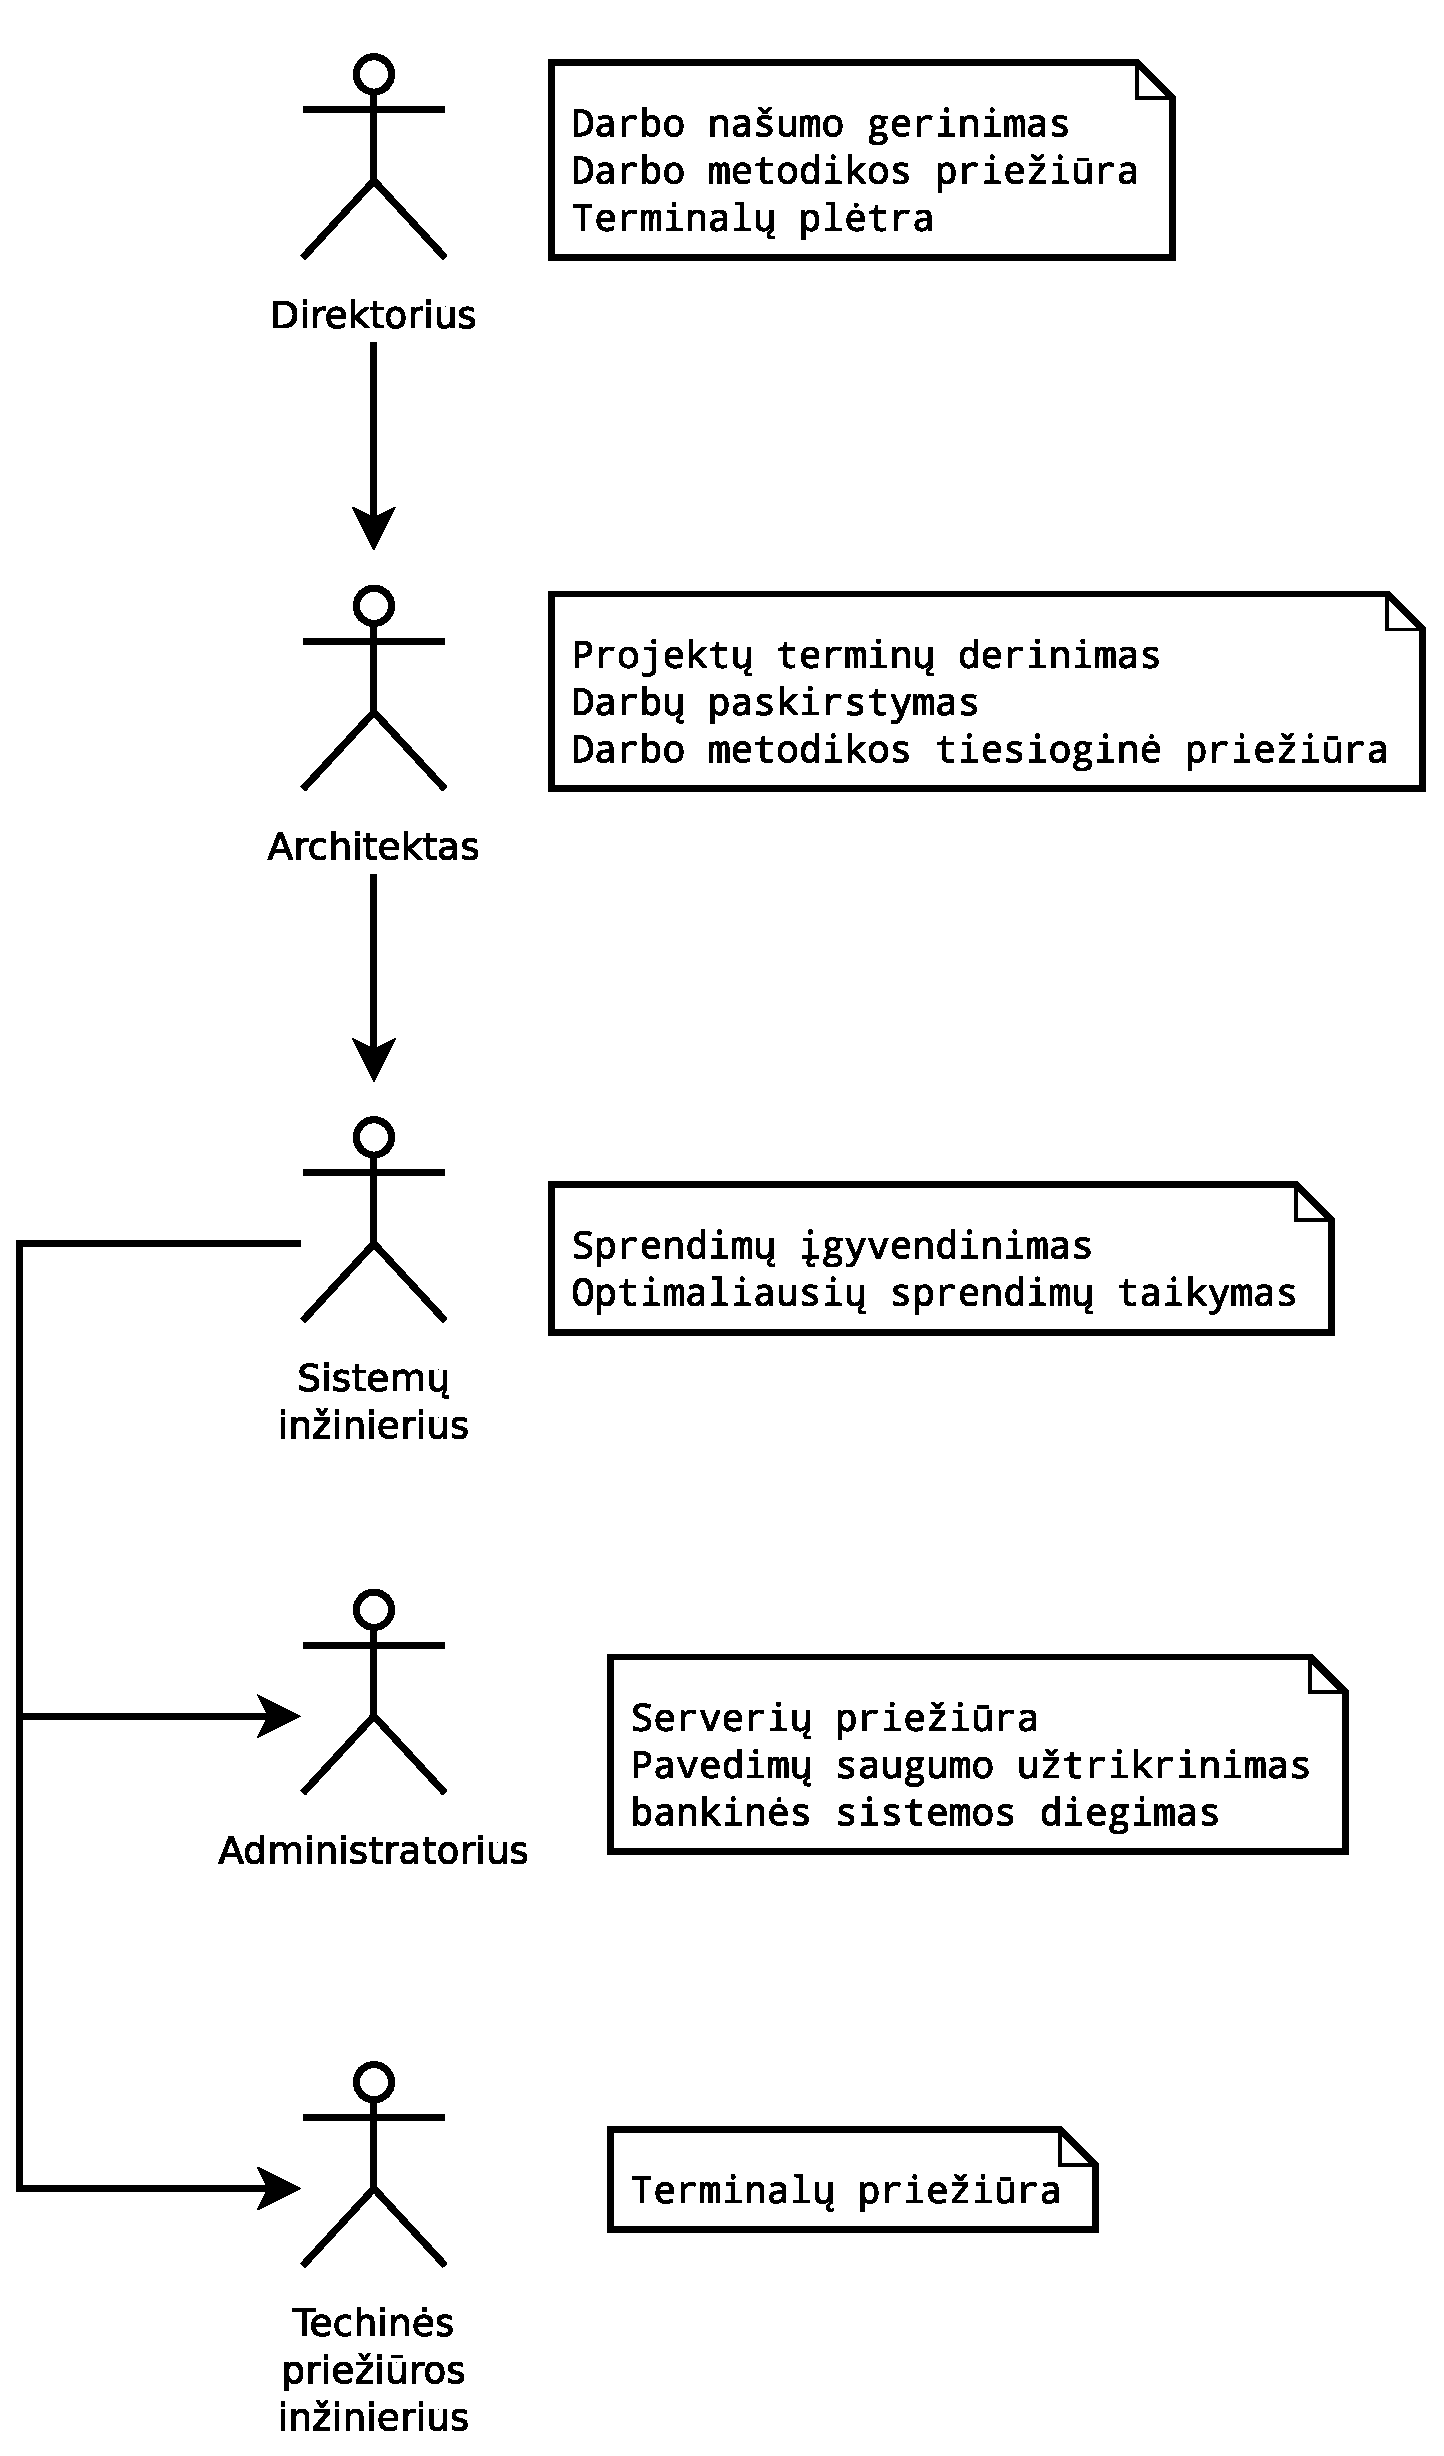
\includegraphics[width=200px]{figures/hierarchija.eps}
                \caption{Nagrinėjamos verslo sistemos organizacinė struktūra.}
                \label{fig:hierarchija}
            \end{figure}

        \subsection{Išvados}

            Laboratorinio darbo metu sumodeliuota verslo sistemos organizacinė struktūra pagal hierarchinius ryšius, pateiktos ribos, kuriose vykdoma analizė. Išvardintos kiekvienos grandines pagrindinės funkcijos ir sąryšiai.

    \section{Laboratorinis darbas nr. 4}

        \subsection{Užduotis}

            Verslo sistemos procesų modeliavimas. Aprašyti bent 3 procesus. Pateikti procesų naudojamus išteklius, proceso veikimo rezultatus, kokius tikslus įgyvendina procesas., kas jį valdo ir t.t. Paprastai tam naudojama klasių arba objektų diagrama. Kiekvienam procesui yra pateikiama veiklos ir/arba sekų diagrama, kurioje detaliai parodyta, kaip vykdomas procesas, kas jį vykdo.

        \subsection{Įvadas}

            Pateikiami tris procesai. Vienas iš procesų yra kliento užklausos siuntimas, atsiskaitymui už paslaugos. Kitas procesas yra sistemos atnaujinimas. Paskutinis pateikiamas procesas yra nuolatinės sistemos versijos atnaujinimas.

        \subsection{Analizė}

            Kliento verslo procesas yra pateikiamas \ref{fig:kliento_verslo_procesas} pav. Sistemos atnaujinimo procesas yra pateikiamas \ref{fig:sistemos_atnaujinimas} pav. Sistemos nuolatinės versijos procesas yra pateikiamas \ref{fig:nuolatines_versijos_modelis} pav.

            \begin{figure}[t]
                \centering
                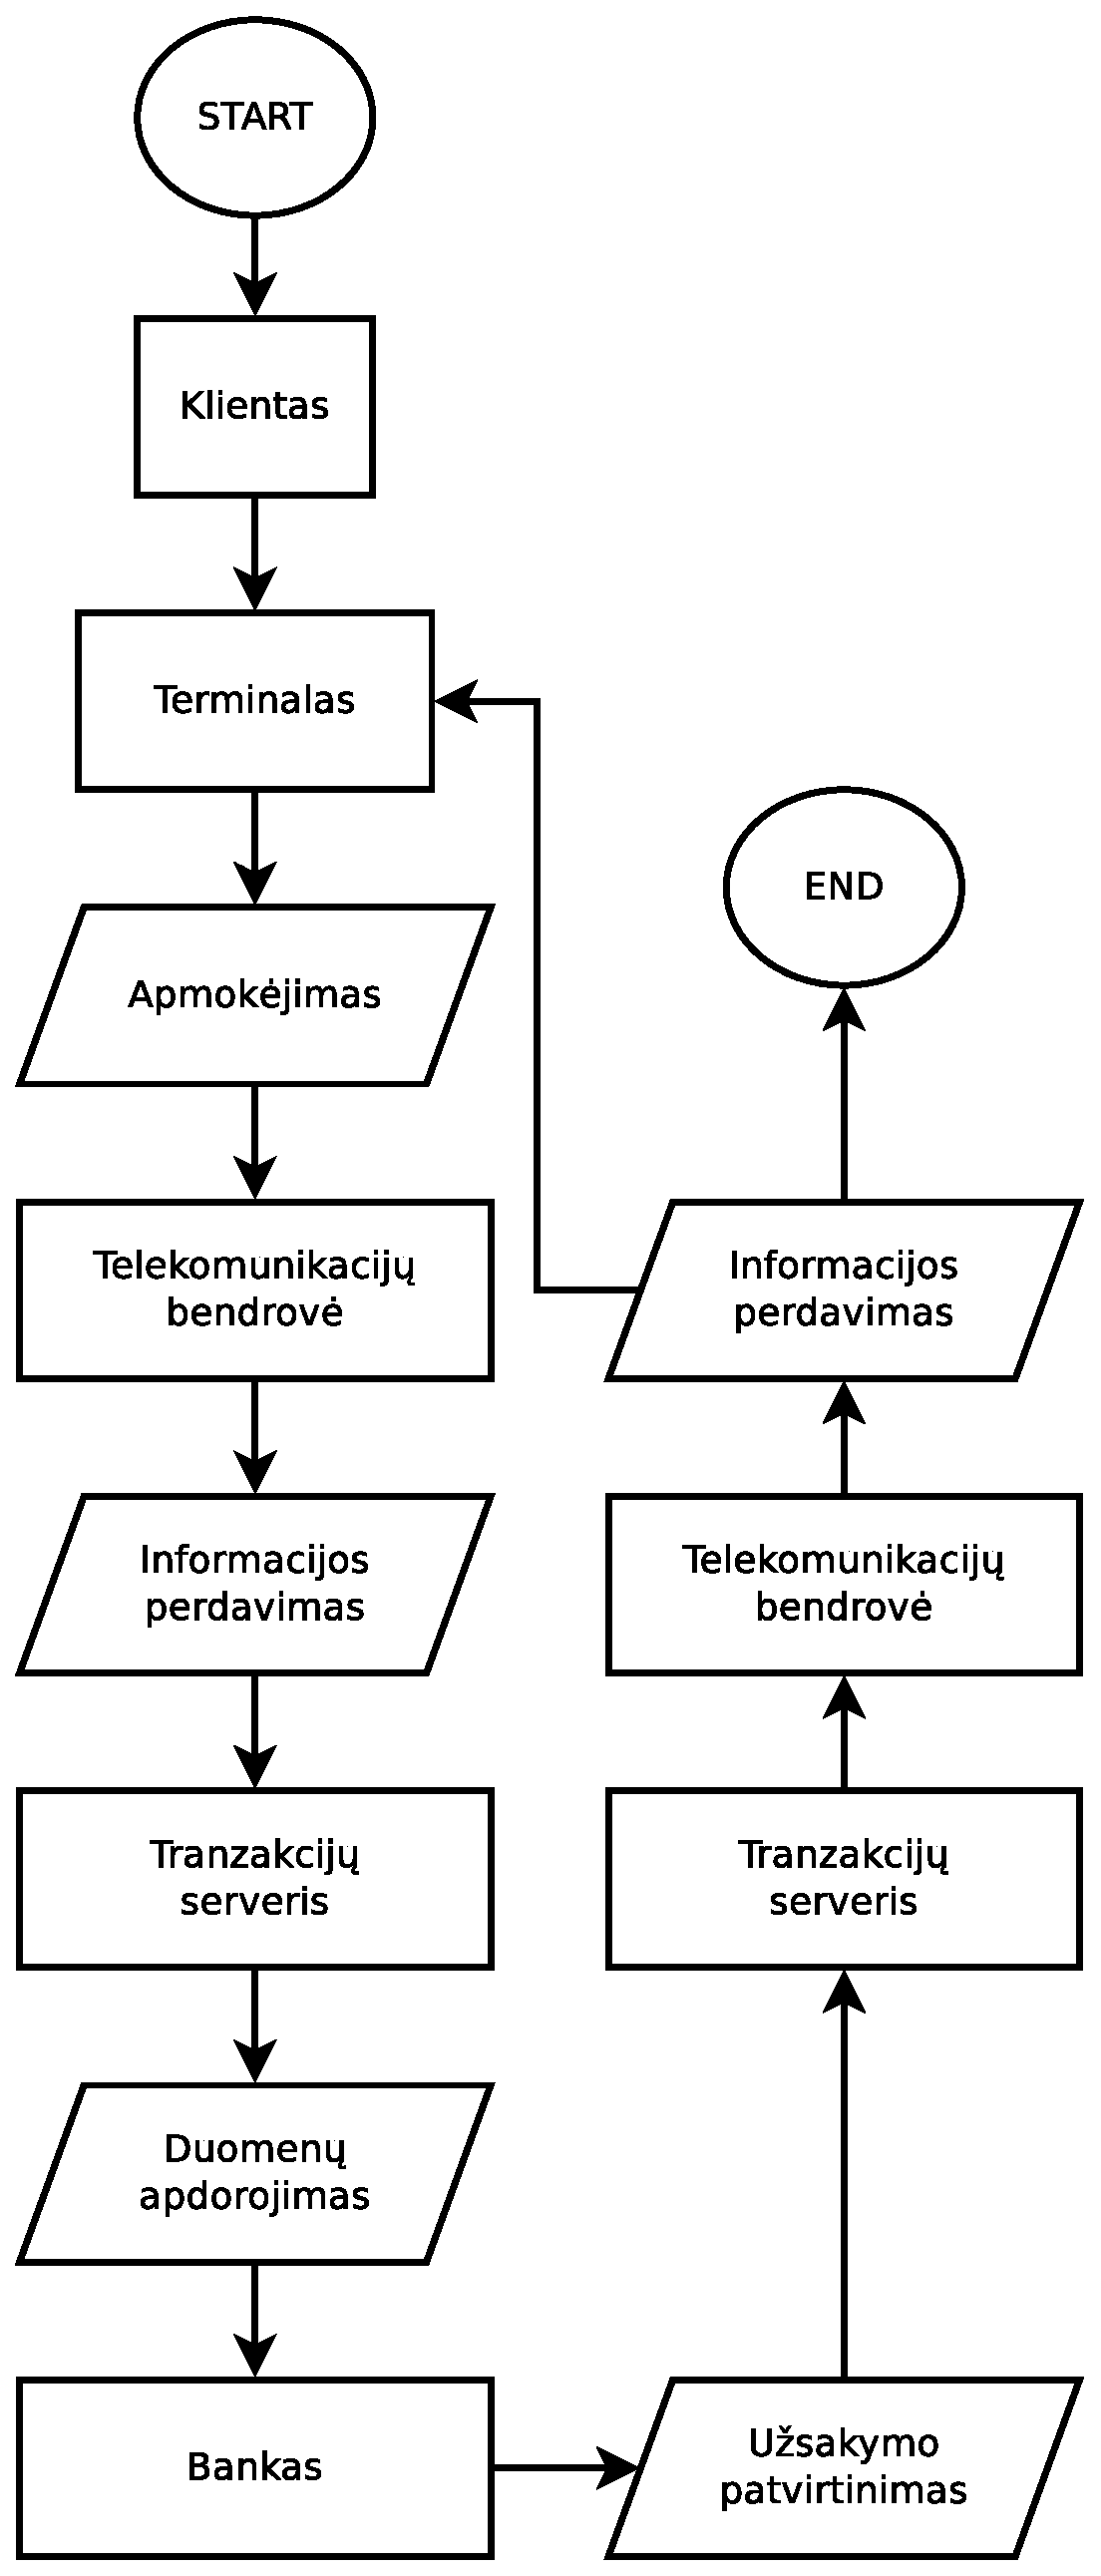
\includegraphics[width=200px]{figures/kliento_verslo_procesas.eps}
                \caption{Kliento verslo sistemos proceso modeliavimas.}
                \label{fig:kliento_verslo_procesas}
            \end{figure}

            \begin{figure}[t]
                \centering
                \includegraphics[width=200px]{figures/sistemos_atnaujinimas.eps}
                \caption{Sistemos atnaujinimas.}
                \label{fig:sistemos_atnaujinimas}
            \end{figure}

            \begin{figure}[t]
                \centering
                \includegraphics[width=200px]{figures/nuolatines_versijos_modelis.eps}
                \caption{Nuolatinės versijos modelis.}
                \label{fig:nuolatines_versijos_modelis}
            \end{figure}

        \subsection{Išvados}

            Laboratorinio darbo metu pateikti 3 verslo procesai, kuriuose dalyvauja analizuojamos verslo sistemos objektai. Visuose procesuose pateikiama sekos diagrama, kurioje detaliai parodyta, kaip vykdomas procesas ir kas jį vykdo.

    \section{Laboratorinis darbas nr. 5}

        \subsection{Užduotis}

            Pateikiamos verslo sistemos užduotys. Kiekvienas užduoties vykdymas parodomas naudojant veiklos ir/arba sekų ir/arba ansamblių diagramas. Kiekvieną užduotį specifikuoti naudojant:

            \begin{itemize}
                \item Užduotis pavadinimą
                \item Tikslą
                \item Sėkmės veiksnius
                \item Sėkmės vertinimo kriterijus
                \item Ypatingas situacijas
                \item Variantus
            \end{itemize}

        \subsection{Įvadas}

            Kiekvienas iš objektų verslo įmonėje turi atlikti jam skirtas užduotis. Užduotis vienaip galima traktuoti kaip tiesioginės ir netiesioginės pareigos. Analizės metu nagrinėjama kiekvieno modelio objekto pagrindinė užduotis, ko būtent reikia, kad užduotis būtų sėkminga. Apžvelgti atvejai, kurie neleidžia tiesiogiai atlikti objekto užduoties.

        \subsection{Analizė}

            Analizei darbo užduočių schema bus panaudota iš prieš tai buvusio laboratorinio darbo. Darbo užduočių schema pateikiama \ref{fig:hierarchija} pav. Iš kiekvieno objekto parinkta viena užduotis ir detaliai išanalizuota. 

            \begin{itemize}
                \item Užduoties pavadinimas
                \begin{itemize}
                    \item Terminalų plėtra
                \end{itemize}
                \item Tikslas
                \begin{itemize}
                    \item Verslo plėtra
                \end{itemize}
                \item Sėkmės veiksniai
                \begin{itemize}
                    \item Sėkmingas bendradarbiavimas su Savivaldybe
                    \item Inovacijos, leidžiančios pigiau suteikti tą pačią paslaugą
                \end{itemize}
                \item Sėkmės vertinimo kriterijai
                \begin{itemize}
                    \item Apyvartos didėjimas
                    \item Darbo vietų didėjimas
                    \item Įmonės apimamo automobilių vietų skaičiaus didėjimas
                \end{itemize}
                \item Ypatingos situacijos
                \begin{itemize}
                    \item Bendradarbiavimo su savivaldybe nutraukimas
                    \item Didelio konkurento į vietinę rinką atėjimas
                \end{itemize}
                \item Variantai
                \begin{itemize}
                    \item Teigiamas arba neigiamas
                \end{itemize}
            \end{itemize}

            \enspace\enspace\enspace

            \begin{itemize}
                \item Užduotis pavadinimas
                \begin{itemize}
                    \item Projektų terminų derinimas
                \end{itemize}
                \item Tikslas
                \begin{itemize}
                    \item Optimaliai paskirstyti laiką
                \end{itemize}
                \item Sėkmės veiksnius
                \begin{itemize}
                    \item Profesionali komanda
                    \item Komanda pilnai supranta kiekvieno stiprumus ir trūkumus, taip sėkmingai skirdama užduotis tarp tų, kurie geriau jas supranta.
                    \item Racionalus 
                \end{itemize}
                \item Sėkmės vertinimo kriterijus
                \begin{itemize}
                    \item Aiškios darbo apimtys
                \end{itemize}
                \item Ypatingas situacijas
                \begin{itemize}
                    \item Darbuotojo liga
                    \item Neplanuotas darbuotojo praradimas
                \end{itemize}
                \item Variantus
                \begin{itemize}
                    \item Terminas bus per trumpas
                \end{itemize}
            \end{itemize}

            \enspace\enspace\enspace

            \begin{itemize}
                \item Užduotis pavadinimas
                \begin{itemize}
                    \item Sprendimų įgyvendinimas
                \end{itemize}
                \item Tikslas
                \begin{itemize}
                    \item Pateikti sprendimą, pagal pateiktą specifikaciją
                \end{itemize}
                \item Sėkmės veiksnius
                \begin{itemize}
                    \item Darbuotojo profesionalumas
                    \item Testų rašymas
                    \item \textit{Design pattern} naudojimas
                \end{itemize}
                \item Sėkmės vertinimo kriterijus
                \begin{itemize}
                    \item Įgyvendintas sprendimas pagal specifikaciją
                    \item Laiku įgyvendintas sprendimas
                \end{itemize}
                \item Ypatingas situacijas
                \begin{itemize}
                    \item Darbuotojo liga
                    \item Specifikacijos pakeitimas
                \end{itemize}
                \item Variantus
                \begin{itemize}
                    \item Užduotis arba įvykdoma arba neįvykdoma
                \end{itemize}
            \end{itemize}

            \enspace\enspace\enspace

            \begin{itemize}
                \item Užduotis pavadinimas
                \begin{itemize}
                    \item Serverių priežiūra
                \end{itemize}
                \item Tikslas
                \begin{itemize}
                    \item Užtikrinti labai mažą \textit{downtime}
                \end{itemize}
                \item Sėkmės veiksnius
                \begin{itemize}
                    \item Naudojama programinė ir operacinė įranga yra gerai pratestuota ir negrąžina netikėtų rezultatų
                \end{itemize}
                \item Sėkmės vertinimo kriterijus
                \begin{itemize}
                    \item Mažas \textit{downtime}
                    \item Esant didelėms apkrovoms, serveris atsako į kiekvieną užklausą
                \end{itemize}
                \item Ypatingas situacijas
                \begin{itemize}
                    \item Serverio lūžimas
                    \item Klaidinga serverio konfigūracija
                    \item Neplanuotas diskų sistemos lūžimas
                \end{itemize}
                \item Variantus
                \begin{itemize}
                    \item Serverio \textit{downtime} ne dėl serverio klaidų, o dėl programuotojo pateikto naujo programinio paketo struktūros ar nenumatytų reikalavimų.
                \end{itemize}
            \end{itemize}

        \subsection{Išvados}

            Laboratorinio darbo metu buvo pateiktos verslo sistemos užduotys, kiekvienas užduoties vykdymas parodytas veiklos diagrama, kuri buvo panaudota iš ankstesnio laboratorinio darbo. Kiekviena užduotis specifikuota naudojant pateiktus reikalavimus.



\end{document}